\newcommand{\AVal}{0.423}
\newcommand{\AEcalVal}{0.387}

\chapter{Event Selection}
\label{evSel}
Most analyses, including this one, are only interested in particle 
interactions that happen relatively rarely during proton collisions.  
Therefore, methods have been developed to sort through all the 
events and select the interesting ones for further study.  
This selection takes place both ``online,'' in real time as the 
detector is running, and ``offline,'' after the previously-selected data has 
been stored.  
%The selection done online is primarily for the purpose of reducing 
%the volume of data enough to store it
The online selection serves primarily for reducing the 
volume of data 
%enough to feasibly store it, 
enough that it can be stored, 
and so it is done centrally. 
In addition, the online selection is fairly general, 
while the offline selection is much more detailed and specific to individual 
analyses, and hence it is mostly done by the user of the data.  


\section{Online}
\label{evSel:online}
The online selection consists mainly of the trigger system, 
described in technical detail in Section~\ref{exp:trigger}.  
%The implementation of the trigger's analysis-oriented f;adsjkl
%is discussed in the following sections, 
%especially the aspects relevant to this analysis.  
The implementation of the trigger system's algorithms 
that are relevant to this analysis 
is discussed in the following sections, 
including both the Level-1 and the High-Level Triggers.  
Both levels reconstruct possible physics objects 
%(in this analysis $e/\gamma$ or electron objects)
and apply criteria to select the interesting events.  
In general, the processing at the Level-1 is quicker 
and coarser in order to sort through a larger volume of data, 
while the High-Level Trigger processing can afford to be 
longer and more thorough because it only deals with 
data not already discarded by the Level-1.  
In addition, as a last step, the information 
from the High-Level Trigger is used to 
group the data into primary datasets
which are used as the basis for the offline selections.  

\subsection{Trigger Eras}
\label{evSel:triggerEras}
%\subsection{Electron Trigger}
%\subsubsection{Electron Algorithms}
%\subsubsection{Trigger Performance}
Since the LHC began taking data the event rate has changed by several orders of magnitude,  
%In order to keep up with the changing rate, 
and the trigger menus have evolved accordingly to deal with the changes.  
Initially, the collision rate was so low that minimum bias triggers ran unprescaled, 
so they were used to take the first analysis data.  
However, the collision rate soon increased to the point where the minimum bias trigger rate became too high
and had to be prescaled, 
and 
%photon 
electromagnetic object %(EM) % Sridhara % COMMENTED
triggers were instead used %instead % , 
to specifically capture events with electron-like objects.  % 
Eventually the 
%photon 
%EM % Sridhara again % COMMENTED in favor of
electromagnetic 
trigger rate at the desired threshold also became too high,
necessitating the extra constraints of the electron trigger at the same threshold.  
The rate for that trigger also increased, so to avoid prescaling the rate or increasing the threshold,
tighter selection criteria were applied to the objects that fired the trigger.  
These criteria are looser than those applied in the course of this analysis and so are not expected
to seriously affect the trigger efficiency for the analysis sample.  


%% TALK ABOUT SOMEWHERE PREVIOUSLY: <strike>TRIGGER MENUS + PRESCALES,</strike> *MINIMUM BIAS*

\subsection{Level-1 Trigger}
\label{evSel:L1}
%\subsubsection{Description of Algorithm}
%Description of egamma algorithm, along with diagrams.  
%The electron-reconstruction algorithm for the Level-1 trigger is implemented in the Regional Calorimeter Trigger (see detector section).
Reconstructing and triggering on an electron with the Level-1 Trigger 
involves information from the calorimeters, processed by 
the Regional Calorimeter Trigger, Global Calorimeter Trigger, and 
Global Trigger.  
Electrons and photons are indistinguishable in the L1 trigger and are therefore 
treated the same, as ``$e/\gamma$'' (or EG) objects.  

The RCT processing was described in detail in 
Section~\ref{exp:RCT}; 
this section provides details on the full-chain processing of $e/\gamma$ triggers.  
The ECAL trigger primitive generation system (TPG) combines the energy deposits 
from a 5x5 square of ECAL crystals into a single energy value corresponding to 
one trigger tower. % and sends it, 
%compressed, to the RCT.  
In addition, for each tower the ECAL TPG calculates a ``fine grain veto'' bit: 
if most of the tower's energy is deposited in a 2x5 strip of crystals, 
then the energy pattern is considered consistent with that of an electron
or photon, 
and the veto bit is not set.  
Otherwise, the veto bit is set.  
% HOW EXACTLY IS SPIKE-KILLING DONE -- FG or zeroed?
Similarly, the HCAL also combines energy deposits into trigger towers; 
however, the HCAL fine grain structure bit is not used in electron-finding.  
The information from the ECAL and HCAL is compressed and sent to the 
Regional Calorimeter Trigger.  
The RCT does the main job of electron-finding using several algorithms, 
detailed in Section~\ref{exp:RCT} and recapped here.  
The decompressed ECAL energy of each trigger tower is examined and 
compared to that of its four adjacent neighbors.  
If the energy of the tower is greater than that of its neighbors, 
it is considered an $e/\gamma$ candidate.  
The candidate energy is set to the energy of the tower in question 
plus that of its highest-energy neighbor.  
However, if the tower's fine grain bit is set, 
or if the ratio of the tower's HCAL energy to ECAL energy is too high, 
it is vetoed as a candidate.  
A candidate is additionally considered ``isolated'' if, 
out of the eight towers directly surrounding it, 
there are five contiguous towers forming an L-shape whose 
energies are low and who pass the fine grain and HCAL/ECAL ratio veto.  
Otherwise, the candidate is ``non-isolated.''  
The RCT sends the collections of isolated and non-isolated candidates to the 
Global Calorimeter Trigger, 
which sends the highest-energy ones to the final step of the L1, the Global Trigger.  
The Global Trigger then applies the criteria determining whether or not 
this event passes the current set of trigger paths,
for example, ``two $e/\gamma$ objects with energy above 10 GeV'' 
or ``one $e/\gamma$ object with energy above 17 GeV.''  
For this analysis, the L1 trigger used only required one $e/\gamma$ 
object, above a threshold which changed from 5 GeV to 8 GeV 
as the luminosity increased (\texttt{L1\_EG5} and \texttt{L1\_EG8}).  
A low threshold is used at the Level-1 Trigger 
to avoid interfering with the performance 
of the higher thresholds used in the High-Level Trigger.  
Efficiency distributions as a function of 
reconstructed supercluster \Et for the 5 and 8 GeV triggers 
are shown in Figure~\ref{fig:L1Effs}, 
using early collision data.  
The efficiency is defined as the fraction of reconstructed electrons 
with \Et in a given bin that caused the given trigger to fire.  
The distributions are divided into barrel-only and endcap-only plots.  
In each case, a high efficiency is not reached until 
the supercluster \Et is several GeV above the Level-1 threshold.  
However, the HLT paths seeded by these triggers require 
a higher value of \Et, 
such that the Level-1 efficiency has already reached the maximum value 
and therefore does not cause a problem.  

% PUT THE PICTURE!!!!   ...?
 \begin{figure}[htb]
  \begin{center}
    \subfloat[\texttt{L1\_EG5}, barrel]{\label{fig:L1Effs5Barrel}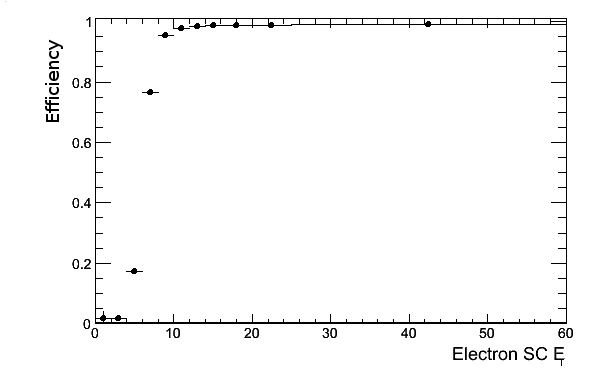
\includegraphics[width=180pt]{Figures/eff_num_ETA_BARREL__SEED_BOTH__TRIG_MATCHED__VS_ELEC_SC_ET__L1_EG5_revised.png}}
    \subfloat[\texttt{L1\_EG5}, endcap]{\label{fig:L1Effs5Endcap}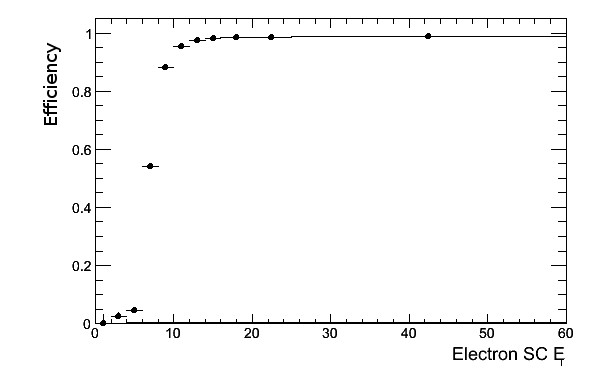
\includegraphics[width=180pt]{Figures/eff_num_ETA_ENDCAP__SEED_BOTH__TRIG_MATCHED__VS_ELEC_SC_ET__L1_EG5_revised.png}}
    \subfloat[\texttt{L1\_EG8}, barrel]{\label{fig:L1Effs8Barrel}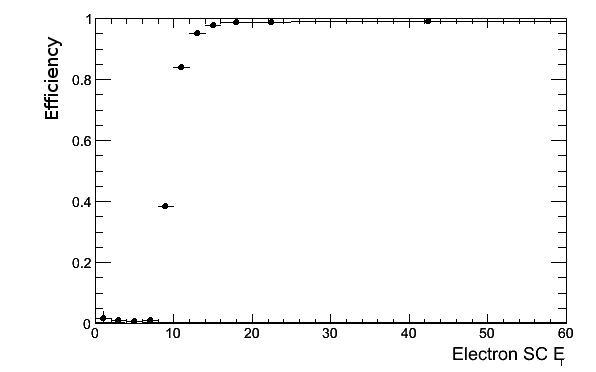
\includegraphics[width=180pt]{Figures/eff_num_ETA_BARREL__SEED_BOTH__TRIG_MATCHED__VS_ELEC_SC_ET__L1_EG8_revised.png}}
    \subfloat[\texttt{L1\_EG8}, endcap]{\label{fig:L1Effs8Endcap}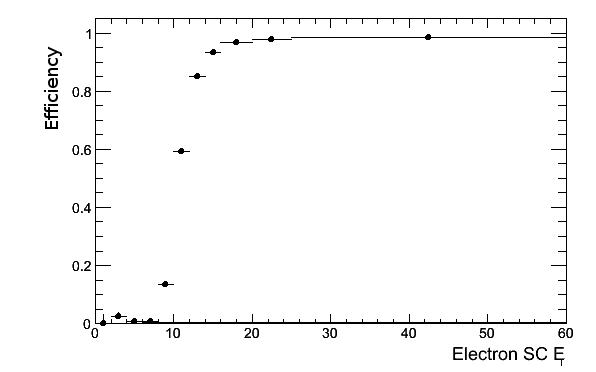
\includegraphics[width=180pt]{Figures/eff_num_ETA_ENDCAP__SEED_BOTH__TRIG_MATCHED__VS_ELEC_SC_ET__L1_EG8_revised.png}}
  \end{center}
  \caption[\fixspacing Efficiency as a function of
  reconstructed supercluster \Et for Level-1 triggers]
  {\fixspacing Efficiency distributions as a function of
  reconstructed supercluster \Et for the Level-1 5 and 8 GeV triggers
  using early collision data.
  The efficiency is defined as the fraction of reconstructed electrons
  with \Et in a given bin that caused the given trigger to fire.
  \subref{fig:L1Effs5Barrel} and \subref{fig:L1Effs5Endcap} show barrel and endcap respectively for 
  \texttt{L1\_EG5}, 
  and \subref{fig:L1Effs8Barrel} and \subref{fig:L1Effs8Endcap} show barrel and endcap for
  \texttt{L1\_EG8}. 
  In each case, a high efficiency is not reached until
  the supercluster \Et is several GeV above the Level-1 threshold.
  }
  \label{fig:L1Effs}
 \end{figure}




%% \subsubsection{Performance}
%% This is where I want to put distributions, resolutions, efficiencies of Level-1 electron/photon objects, 
%% when/if I make/get them.  Made some with old code a long time ago, but those are outdated.  
%% Redo my own?

%% Figures: Trigger Electron/Photon Pt, eta, phi spectra for L1, Fig. \ref{fig:L1TriggerObjectSpectra}

%%  \begin{figure}[htb]
%%   \begin{center}
%%     
\includegraphics[width=360pt]{CMS-BW.pdf}
%%   \end{center}
%%   \caption[\fixspacing Trigger Electron/Photon Pt, eta, phi spectra for L1]{\fixspacing Trigger Electron/Photon Pt, eta, phi spectra for L1.}
%%   \label{fig:L1TriggerObjectSpectra}
%%  \end{figure}


%% Figures: \DR for L1 trigger object matching, Fig. \ref{fig:L1TriggerObjectDeltaR}

%%  \begin{figure}[htb]
%%   \begin{center}
%%     
\includegraphics[width=360pt]{CMS-BW.pdf}
%%   \end{center}
%%   \caption[\fixspacing \DR for L1 trigger object matching to offline]{\fixspacing \DR for L1 trigger object matching to offline-reconstructed objects.}
%%   \label{fig:L1TriggerObjectDeltaR}
%%  \end{figure}

%% Figures: L1 trigger Pt resolution plots using offline reference, Fig. \ref{fig:L1TriggerObjectResolutions}

%%  \begin{figure}[htb]
%%   \begin{center}
%%     
\includegraphics[width=360pt]{CMS-BW.pdf}
%%   \end{center}
%%   \caption[\fixspacing L1 trigger Pt resolution plots using offline reference]{\fixspacing L1 trigger Pt resolution plots using offline reference.}
%%   \label{fig:L1TriggerObjectResolutions}
%%  \end{figure}

%% Figures: L1 trigger electron/photon efficiency turn on using offline reconstructed electrons and MC, Fig. \ref{fig:L1TriggerObjectEfficiencies}

%%  \begin{figure}[htb]
%%   \begin{center}
%%     
\includegraphics[width=360pt]{CMS-BW.pdf}
%%   \end{center}
%%   \caption[\fixspacing L1 trigger electron/photon efficiency turn on using offline reconstructed electrons and MC]{\fixspacing L1 trigger electron/photon efficiency turn on using offline reconstructed electrons and MC.}
%%   \label{fig:L1TriggerObjectEfficiencies}
%%  \end{figure}


\subsection{High-Level Trigger}
\label{evSel:HLT}

%\subsubsection{Description of Algorithms}
%Description of algorithms.

The algorithms used to reconstruct trigger objects 
in the High-Level Trigger are the same as those 
used in the offline analysis and are described in Chapter~\ref{evReco}.  
However, because of timing considerations, 
the algorithms are combined and configured differently at the HLT.  
The HLT has a limited amount of time in which to 
make a keep/discard decision for a given event 
in order to keep up with the flow of events.  
Therefore the algorithms are optimized for the best 
performance in the shortest time, 
which in practice means fewer steps and less 
complexity than the implementation at the offline level, 
where no such constraint exists.  
In particular, while the offline-reconstructed 
electron collection 
includes tracker-driven electrons, 
those reconstructed at the HLT are ECAL-driven only, 
and the supercluster reconstruction algorithm 
(Section~\ref{evReco:SC}) uses 
a lower number of steps in the search process.  
Also, the size of the windows in which to search for 
hits in the pixel-matching part of the 
reconstruction (Section~\ref{evReco:pixMatch}) 
is larger than that used offline, 
to guarantee a high efficiency.  

%% However, these algorithms are used in different ways at the HLT 
%% because of differences in performance considerations.  
%% Namely, the algorithms as implemented in the HLT tend to be 
%% configured to require 
%% fewer steps and less complexity than at the offline level.  
%% This includes in particular timing considerations.  
%% The HLT has a time constraint in which to make its decision 
%% to save or discard an event.  

%% Another theme: evolution of triggers, from photon to electron to calo eID to full eID/isol, 
%% for purpose of keeping rate down (manageable) as L goes up.  

%%    * short summary of each sort of thing?  (with reference to event reco chapter)
%% YES, just the things that are used in the relevant paths.  
%% have short mentions also of e.g. eid vars and give reference to future section


%% things common to all paths used: L1 match, SC reco, spike, et cut

%% somewhere say how even with additions of criteria, 
%% less complicated than offline still, and show why

The luminosity increase and consequent evolution of trigger menus 
described in Section~\ref{evSel:triggerEras} required incremental changes 
in the definitions of the current HLT paths.  
However, a few requirements remained common to all the paths used.  
In particular, the execution of each path begins by taking 
the Level-1 objects that passed the given L1 seed path 
and retrieving the information from the ECAL regions % make sure we're in context of MY HLT paths
around those objects.  
From this information, 
clusters of energy deposits are identified, 
and clusters having too narrow a spatial distribution are 
rejected as being spikes.  
%........???????
The trigger paths used in this analysis, 
shown in chronological order in Table~\ref{TableTriggerPaths}, 
all required (at least) one 
$e/\gamma$ or electron candidate above a certain energy threshold, 
with possible other criteria applied to the candidate as well.%, 
%depending on the path.  

%Table of triggers used
\begin{table}[htbp]
%  \centering
  \begin{center}
    \caption[Trigger paths used to select data]
    {\fixspacing Trigger paths used to select data, 
    in chronological order of use. 
    See text for explanation of path names.  
    }
    \label{TableTriggerPaths}
%    \begin{tabular}[]{ | l | c | c | }
    \begin{tabular}[]{ | l | c | }
      \hline
      Trigger & L1 Seed \\ \hline \hline
      HLT\_Photon15\_Cleaned\_L1R & L1\_EG5 \\ \hline
      HLT\_Ele15\_LW\_L1R & L1\_EG8 \\ \hline
      HLT\_Ele15\_SW\_L1R & L1\_EG8 \\ \hline
      HLT\_Ele15\_SW\_CaloEleId\_L1R & L1\_EG8 \\ \hline
      HLT\_Ele17\_SW\_CaloEleId\_L1R & L1\_EG8 \\ \hline
      HLT\_Ele17\_SW\_TightEleId\_L1R & L1\_EG8 \\ \hline
      HLT\_Ele17\_SW\_TighterEleIdIsol\_L1R & L1\_EG8 \\ \hline
    \end{tabular}
  \end{center}
\end{table}

The paths are named according to the following considerations.  
Initially, the LHC collision rate was low enough that loose 
requirements and low thresholds could be used without 
overwhelming the system.  
The first trigger used did not require any matches to 
hits in the pixel part of the tracker, 
in contrast to all subsequent trigger paths used -- 
without tracking requirements, it was by definition a 
``Photon'' trigger, 
as opposed to the ``Electron (Ele)'' triggers.  
The designation ``Cleaned'' means that a spike-cleaning 
algorithm was in place, as well.  
%In addition, 
After a few menu iterations 
the energy threshold applied to the candidate, 
designated by the number in the path name,  
increased from 15 GeV to 17 GeV.  
The size of the window used to search for potential pixel 
matches also decreased, from ``large-window'' ($LW$) 
to ``startup-window'' ($SW$). %, 
%and various further criteria were applied to 
Later, further criteria were applied to 
the shape of the total energy deposit (\sieie, $H/E$); %and 
since this information comes only from the calorimeter, 
paths with such constraints have ``Calo'' in their name.  
Later paths included additional criteria, 
on the quality of the match between the energy cluster and the track 
that make up the electron (\detain, \dphiin), 
and were designated as ``Tight'' or ``Tighter'' according 
to the stringency of their constraints.  
Finally, constraints were added for the amount of energy surrounding 
the electron candidate, or ``isolations'' 
designated by ``Isol'' in the path name.  
These further criteria are described in more detail in 
Section~\ref{evSel:elec}; 
%Sections~\ref{evSel:eid}~and~\ref{evSel:isol}; 
in the current section it is sufficient to say that they 
were added in steps to the trigger paths to gradually tighten the 
selection.  
Efficiency distributions for an early trigger are shown 
in Figure~\ref{fig:HLTEffs}.  
In this case, the efficiency is defined as the fraction of reconstructed electrons
with \Et in a given bin that caused the given trigger to fire. 
Figure~\ref{fig:HLTEffsPhot15Barrel} shows the efficiency for 
the barrel, 
while Figure~\ref{fig:HLTEffsPhot15Endcap} is for the endcap 
(the empty bin is due to lack of statistics).  
The trigger reaches maximum efficiency well below the energy 
threshold used in the offline analysis, 
so the inefficiency at the ``turn-on'' does not affect the offline analysis.  

However, the efficiencies for the triggers used in this analysis 
were determined using the tag-and-probe method, detailed in 
Section~\ref{evSel:eff}.  
The results for each of the triggers are also 
given in that section.  

 \begin{figure}[htb]
  \begin{center}
    \subfloat[Barrel]{\label{fig:HLTEffsPhot15Barrel}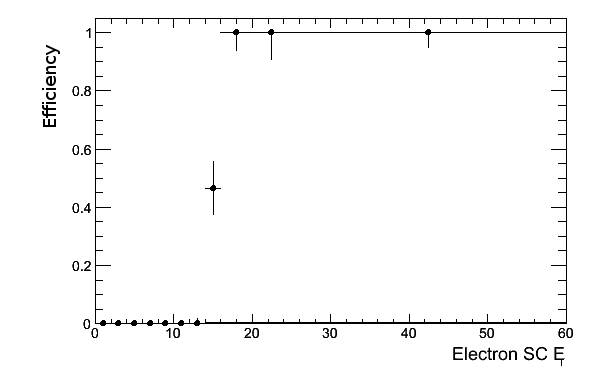
\includegraphics[width=180pt]{Figures/eff_num_ETA_BARREL__SEED_BOTH__TRIG_MATCHED__VS_ELEC_SC_ET__HLT_PHOT15_revised.png}}
    \subfloat[Endcap]{\label{fig:HLTEffsPhot15Endcap}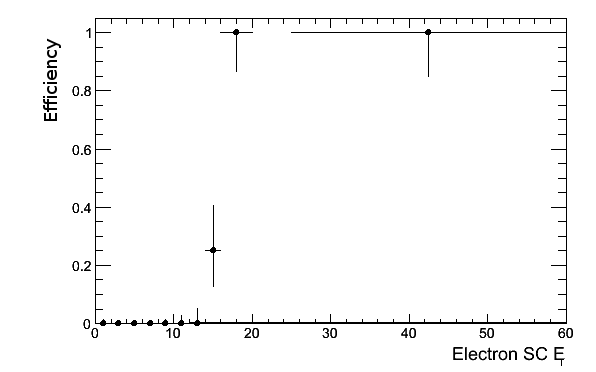
\includegraphics[width=180pt]{Figures/eff_num_ETA_ENDCAP__SEED_BOTH__TRIG_MATCHED__VS_ELEC_SC_ET__HLT_PHOT15_revised.png}}
  \end{center}
  \caption[\fixspacing Efficiency as a function of
  reconstructed supercluster \Et for an early HLT trigger]
  {\fixspacing Efficiency distributions as a function of
  reconstructed supercluster \Et for an early HLT trigger 
  using collision data, \texttt{HLT\_Phot15\_L1R}.
  The efficiency is defined as the fraction of reconstructed electrons
  with \Et in a given bin that caused the given trigger to fire.
  \subref{fig:HLTEffsPhot15Barrel} and \subref{fig:HLTEffsPhot15Endcap} 
  show barrel and endcap respectively. 
  The empty bin in \subref{fig:HLTEffsPhot15Endcap} 
  is due to lack of events in that bin.  
  }
  \label{fig:HLTEffs}
 \end{figure}



%% Basically the same as reco algo's, but with fewer steps and stuff to save time.  
%% Do reduced version (and reference event reconstruction chapter) and 
%% explain differences.  
%% Also explain anything particular to HLT -- like farm, timing, etc 
%% (although maybe that stuff should go in detector chapter).  

%ALSO make these trigger plots.  


%% e/gamma stuff: they added a 1/E - 1/p filter since the last time I did
%% egamma HLT stuff.  probably also added other stuff.  
%% READ UP ON.  Useful-looking talk on egamma trigger strategy 
%% from alessio linked from SWGuideEgammaHLT


%% THEME FOR HLT: like offline, but optimized for good timing (not critical issue offline).  


%% already in reco chapter:

%%    * ecal reco -- rec hits

%%    * spike cleaning based on timing and shape

%%    * track reco, like KF and GSF

%%    * electron reco

%%       * ecal-driven: SC's from BC's (both algos used), pixel-hit matching to make seeds, then make tracks from them

%%       * tracker-driven: 

%% SO, HLT doesn't use tracker-driven stuff, just ECAL-driven








%% \subsubsection{Performance}
%% Distributions, resolutions, efficiencies of HLT electron/photon objects.


%% Figures: Trigger Electron/Photon Pt, eta, phi spectra for HLT, Fig. \ref{fig:HLTriggerObjectSpectra}

%%  \begin{figure}[htb]
%%   \begin{center}
%%     
\includegraphics[width=360pt]{CMS-BW.pdf}
%%   \end{center}
%%   \caption[\fixspacing Trigger Electron/Photon Pt, eta, phi spectra for HLT]{\fixspacing Trigger Electron/Photon Pt, eta, phi spectra for HLT.}
%%   \label{fig:HLTriggerObjectSpectra}
%%  \end{figure}


%% Figures: \DR for HLT trigger object matching, Fig. \ref{fig:HLTriggerObjectDeltaR}

%%  \begin{figure}[htb]
%%   \begin{center}
%%     
\includegraphics[width=360pt]{CMS-BW.pdf}
%%   \end{center}
%%   \caption[\fixspacing \DR for HLT trigger object matching to offline]{\fixspacing \DR for HLT trigger object matching to offline-reconstructed objects.}
%%   \label{fig:HLTriggerObjectDeltaR}
%%  \end{figure}

%% Figures: HLT trigger Pt resolution plots using offline reference, Fig. \ref{fig:HLTriggerObjectResolutions}

%%  \begin{figure}[htb]
%%   \begin{center}
%%     
\includegraphics[width=360pt]{CMS-BW.pdf}
%%   \end{center}
%%   \caption[\fixspacing HLT trigger Pt resolution plots using offline reference]{\fixspacing HLT trigger Pt resolution plots using offline reference.}
%%   \label{fig:HLTriggerObjectResolutions}
%%  \end{figure}

%% Figures: HLT trigger electron/photon efficiency turn on using offline reconstructed electrons and MC, Fig. \ref{fig:HLTriggerObjectEfficiencies}

%%  \begin{figure}[htb]
%%   \begin{center}
%%     
\includegraphics[width=360pt]{CMS-BW.pdf}
%%   \end{center}
%%   \caption[\fixspacing HLT trigger electron/photon efficiency turn on using offline reconstructed electrons and MC]{\fixspacing HLT trigger electron/photon efficiency turn on using offline reconstructed electrons and MC.}
%%   \label{fig:HLTriggerObjectEfficiencies}
%%  \end{figure}


\subsection{Primary Datasets}
\label{evSel:PD}
The final step done centrally is the grouping of events passing similar 
HLT paths into primary datasets for storage.  
For example, in early running, all events passing a minimum-bias trigger 
were put into the MinimumBias dataset.  
Once the event rate increased and physics triggers fired more often, 
events were put into more specific datasets such as 
EG for all events passing $e/\gamma$ (electron or photon) triggers, 
or later, Electron for all events specifically passing 
electron triggers.  
These primary datasets are the groupings of stored data 
that the offline analyses begin with.  
The specific datasets used for this analysis are given in 
Table~\ref{TableDatasets}.  

\begin{table}[htbp]
%  \centering
  \begin{center}
    \caption{\fixspacing Primary datasets used in this analysis.}
    \label{TableDatasets}
%    \begin{tabular}[]{ | l | c | c | }
    \begin{tabular}[]{ | l | }
      \hline
      Dataset  \\ \hline \hline
      /EG/Run2010-Dec22ReReco\_v1/AOD  \\ \hline
      /Electron/Run2010b-Dec22ReReco\_v1/AOD  \\ \hline
    \end{tabular}
  \end{center}
\end{table}

\clearpage
\section{Offline}
\label{evSel:offline}
%Dataset (trig requirements), good vertex selection, etc
The offline selection consists of any criteria applied to the data 
after it has already been stored, 
i.e.\ criteria applied to an already-existing primary dataset.  
This analysis uses data from two consecutive primary datasets: 
the EG dataset gathered during earlier data-taking 
(Run2010A, from run 135821 to run 144114), 
and the Electron dataset from later data-taking 
(the Run2010B era, runs 146240 to 149711).  
In addition, it 
%was 
is 
required that the primary vertex of 
each event be ``good'': 
that is, within 24 cm of the nominal interaction point 
in the longitudinal direction
and 2 cm in the transverse direction, 
and having a minimum of 4 degrees of freedom (called NDOF),
which is a measure of the quality of the vertex fit.  %EXPLAIN WHAT THIS MEANS MORE?
More detailed selections 
%were made on 
are applied to 
the event contents, 
which will be discussed in the following sections.  
The electrons in these events 
%were 
are 
required to pass 
a series of criteria to determine ``good'' electrons.  
Finally, specific selections 
%were 
are 
made on the 
characteristics of the event as a whole 
in order to get the final collection of \Zee candidate 
events.  

\subsection{Electron Selection}
\label{evSel:elec}
The electron selection starts with the full set of objects reconstructed as electrons, 
%i.e. ECAL energy deposits with nearby tracks.  
i.e.\ ECAL energy deposits (superclusters, see Section~\ref{evReco:SC}) matched with nearby tracks.  
The objects in this collection are not necessarily real electrons 
%but energy deposits consistent with those from electrons at a low-level.  
but are consistent with the electron signature at a low level.  
%(talk about def of GSF electron etc so know what kinds of cuts have already been applied)   % to be done in eventReconstruction!
In order to select the reconstructed objects most likely to be real electrons from a Z, 
sets of further conditions are applied.  
%First electrons are matched to trigger objects passing an egamma trigger with a Level-1 threshold of 5 GeV.  
First the electrons are required to be within the $\eta$ region of ECAL in which 
they can be fully measured, in the barrel, $0 < |\eta| < 1.4442$, 
and in the endcap, $1.566 < |\eta| < 2.5$.  
A 25-GeV cut on the supercluster transverse energy is applied,
followed by a set of cuts designed to reject electrons from photon conversions.  
Another set of cuts aims to distinguish real electrons from other energy deposits which may mimic electrons, 
and finally a set of cuts to make sure the electron is isolated, 
i.e.\ not part of a jet unrelated to the Z.  

%All the different wp's for different purposes and efficiencies.  WP95 looser than trigger cuts by the end!  put other reasons too for wp80
The CMS vector boson analysis team created several different electron selections of varying 
%tightness of cuts,
cut tightness,
based on a given efficiency of the cuts \cite{CMSWZ}.  % ref to iterative algo stuff?
A tighter selection in general results in a purer sample of true electrons, but throws away many more
real electrons than a looser selection.  
These ``working points'' have target efficiencies ranging from 95\%-efficient at the loosest (WP95) to 60\% at the tightest (WP60).  
For early data-taking the WP95 and WP80 selections were chosen as the baseline selections for the \Zee and \Wenu analyses, respectively.
As more data accumulated, it became clear that WP80 provided better performance than WP95 for the \Zee analysis, as well.  
A deciding factor in the switch was the fact that the evolving trigger paths eventually used selections that were
tighter than those used in the offline (WP95) analysis.  
This analysis uses the WP80 set of cuts for the complete dataset.  

%The selection cuts are displayed in the following cuts applied only to simulated data.  
The plots in the following sections showing the distributions and cut values 
only display simulated data.  
The QCD Monte Carlo sample has effective electron isolation cuts already applied, 
so until the corresponding selection cuts are applied to data, 
the data does not agree with the Monte Carlo distributions.  
However, after all cuts have been applied the agreement is good; 
this will be demonstrated in a later section.  
All results plots include the data distributions.  

%ETA AND ET CUTS!!!

\subsubsection{Conversion Rejection}
\label{evSel:convRej}
The conversion rejection step of the electron selection aims 
to eliminate photons that have converted into electron pairs.  
Several variables have been chosen to distinguish between 
conversions and prompt electrons 
(electrons from the interaction of interest), 
focusing on the track properties.  
Since prompt electrons are expected to hit the first layer of the tracker, 
any electron-associated track that is missing initial hits 
can be rejected as a conversion that occurred within the tracker.  
The looser requirements of the 95\%-efficient working point 
allow an electron to have one missing hit;
tighter working points such as WP80 require zero missing hits.  
Figure~\ref{fig:MissHitsConvRejVars} shows the number 
of missing hits for each electron.  
In addition, the conversion rejection algorithm searches 
for candidate electron-pair partner tracks, 
i.e. track pairs that appear to come from the same point.  
Every electron track is compared to all opposite-charge tracks 
within a $\Delta R$ cone of 0.3, and two values are calculated: 
a measure of the difference in the angles in the r-z plane 
between the two tracks (\dCotTheta, Figure~\ref{fig:DCotConvRejVars}), 
and the distance of closest approach between the two tracks 
in the x-y plane ($dist$, Figure~\ref{fig:DistConvRejVars}).  
Electron pairs from conversions are expected 
to have low values for both quantities, 
since both electron tracks begin at the point of conversion 
and initially have the same direction as the converting photon.  
The WP80 requirements apply a threshold at 0.02 for both quantities.  
The selection is such that an electron candidate 
that fails both the missing hits cut 
and one of the other cuts is rejected as a conversion.  
This way a single anomalous measurement does not 
result in a true electron being rejected.  
%The 95-percent efficient working point is looser than the other working points in that it does not apply cuts on these quantities.  
%The other working points reject electrons having a value of less than 0.02 for both.  
%If an electron track corresponds to a track pair having values below that threshold for both variables, 
%it is assumed to be a conversion and is rejected.  

 \begin{figure}[htb]
  \begin{center}
    \subfloat[Missing Hits]{\label{fig:MissHitsConvRejVars}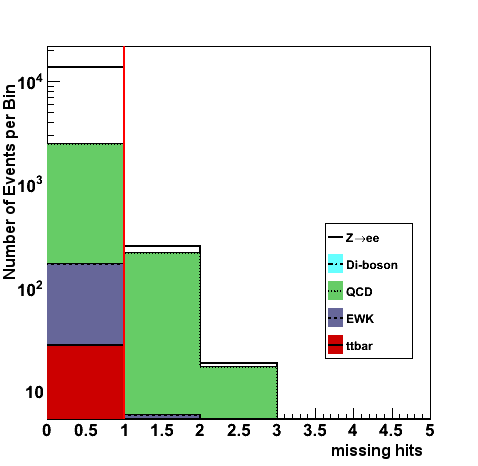
\includegraphics[width=180pt]{Figures/missHits-14Apr11-revised-04Jul11.png}}
    \subfloat[$\Delta\cot\theta$]{\label{fig:DCotConvRejVars}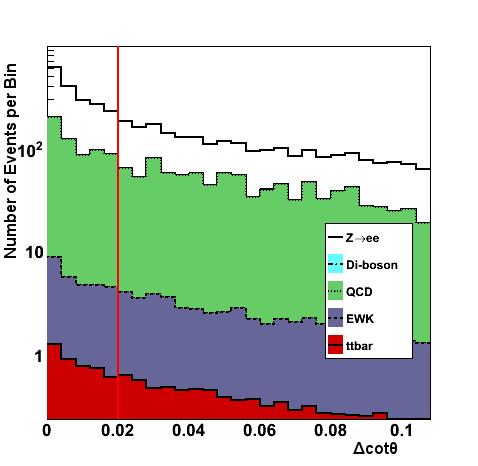
\includegraphics[width=180pt]{Figures/dCotTheta-14Apr11-revised-04Jul11.png}}
    \subfloat[Dist]{\label{fig:DistConvRejVars}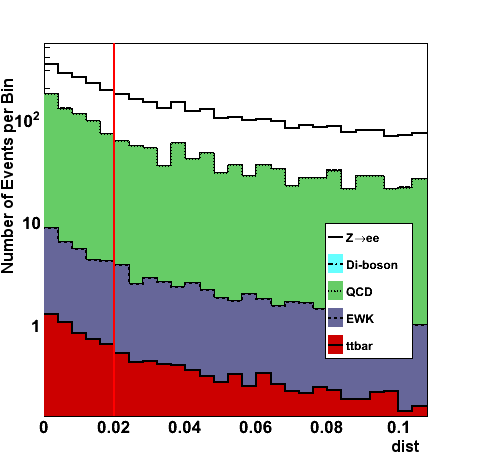
\includegraphics[width=180pt]{Figures/dist-14Apr11-revised-04Jul11.png}}
  \end{center}
  \caption[\fixspacing Conversion rejection variables after \Et cut]
  {\fixspacing Conversion rejection variables after \Et cut: 
  \subref{fig:MissHitsConvRejVars} the number of missing hits in the tracker, 
  \subref{fig:DCotConvRejVars} the value of $\Delta\cot\theta$ 
  between the electron track and any partner track, and 
  \subref{fig:DistConvRejVars} $dist$, 
  the distance of closest approach between the two tracks. 
  The solid line against the white background shows the signal sample; 
  the shaded areas with varied linestyles show the backgrounds. 
  The vertical line shows where the cut was made.  
  }
  \label{fig:ConvRejVars}
 \end{figure}


\subsubsection{Electron Isolation}
\label{evSel:isol}
%It is expected that the products of a Z decay will not 
%exit the interaction region  
%in the vicinity of many other particles, 
%since the Z decay products are not part of a jet. 
The electrons from a Z decay are not expected to end up 
close to many other particles in the detector, 
since they are not produced as part of a jet.  
%We want 
The object is to select those real electrons that are most likely to be prompt decay products,
not those that come from some secondary interaction with many other end products.  
Therefore 
%we apply 
a set of cuts 
is applied 
requiring little detector activity 
in the area immediately surrounding the reconstructed electron.  
These so-called isolation cuts look at the energy deposits 
in the electromagnetic and hadronic calorimeters separately,
as well as the total \pt of neighboring tracks, 
within specified \DR cones around the electron-associated deposit/track.  
These energies are divided by the \pt of the electron itself to arrive at a relative value,
which allows for higher-energy particles that may deposit more energy in the surrounding area.  
The thresholds for each of the three types of isolation are set separately for barrel and endcap, 
because there is more material in front of the endcap, 
causing the electron energy to be more spread out.  
The thresholds are given in Table \ref{TableEisoCuts}.  
Plots of the separate isolation distributions for both barrel and endcap 
are shown after 
%previously-applied selection 
the conversion rejection 
cuts in 
Figure~\ref{fig:trkElecIsoVars} for track isolation, 
Figure~\ref{fig:ecalElecIsoVars} for ECAL isolation, and 
Figure~\ref{fig:hcalElecIsoVars} for HCAL isolation.  

%Conditions to require that electrons found are isolated, i.e. not contained in a jet with other particles.  
%We want (``prompt''?) electrons that come directly from the Z, 
%not from some other interaction with lots of other end products packaged along with the electron.  


%%%%  ISOLATION VALUES

\begin{table}[htbp]
%  \centering
  \begin{center}
    \caption[WP80 thresholds for relative isolation]
    {\fixspacing WP80 thresholds for relative isolation.
    The value of each type of isolation (ECAL, HCAL, track) 
    is divided by the electron's \pt, and the result is 
    required to be below the threshold.  
    }
    \label{TableEisoCuts}
    \begin{tabular}[]{ | l | c | c | }
      \hline
      Cut variable & Barrel & Endcap  \\ \hline \hline
      Track & 0.09 & 0.04 \\ \hline
      ECAL & 0.07 & 0.05  \\ \hline
      HCAL & 0.10 & 0.025  \\ %\hline
%      $ H/E $ & 0.04 & 0.025  \\
      \hline
    \end{tabular}
  \end{center}
\end{table}


%%%% ISOLATION DISTROS

 \begin{figure}[htb]
  \begin{center}
    \subfloat[Barrel]{\label{fig:trkBarrelElecIsoVars}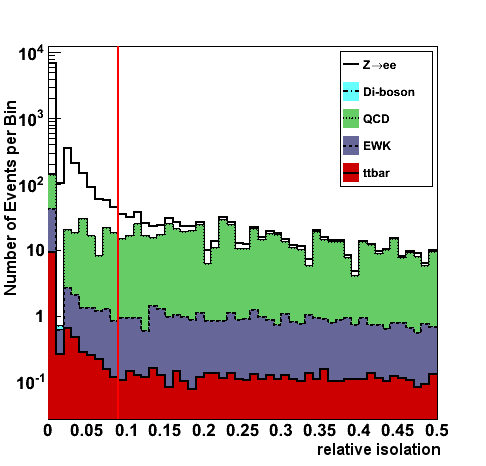
\includegraphics[width=180pt]{Figures/trkIso-barrel-14Apr11-revised-04Jul11.png}}
    \subfloat[Endcap]{\label{fig:trkEndcapElecIsoVars}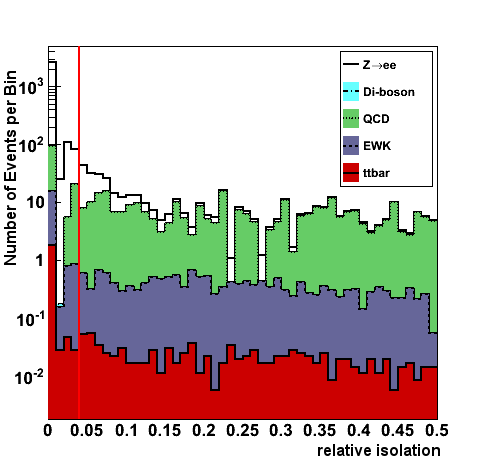
\includegraphics[width=180pt]{Figures/trkIso-endcap-14Apr11-revised-04Jul11.png}}
  \end{center}
%  \caption[\fixspacing Electron tracker isolation variables before respective cuts]
%  {\fixspacing Electron tracker isolation variables before respective cuts.}
  \caption[\fixspacing Electron tracker isolation variables after \Et and conversion rejection cuts]
  {\fixspacing Electron tracker isolation variables after \Et and conversion rejection cuts, for %. 
  \subref{fig:trkBarrelElecIsoVars} barrel and 
  \subref{fig:trkEndcapElecIsoVars} endcap.  
  Relative tracker isolation is equal to the sum of the \pt of tracks 
  in a cone around the electron, divided by the electron's \pt.  
  The solid line against the white background shows the signal sample; 
  the shaded areas with varied linestyles show the backgrounds. 
  The vertical line shows where the cut was made.  
  }
  \label{fig:trkElecIsoVars}
 \end{figure}



 \begin{figure}[htb]
  \begin{center}
    \subfloat[Barrel]{\label{fig:ecalBarrelElecIsoVars}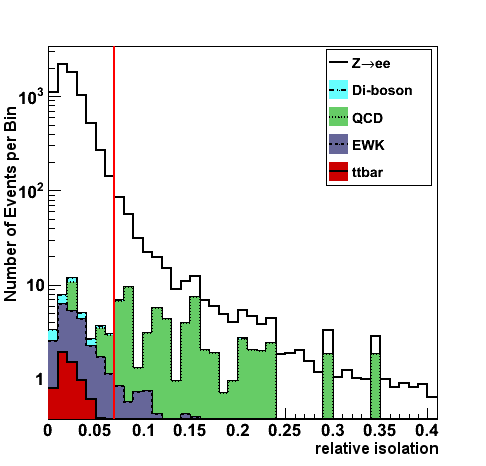
\includegraphics[width=180pt]{Figures/ecalIso-barrel-14Apr11-revised-04Jul11.png}}
    \subfloat[Endcap]{\label{fig:ecalEndcapElecIsoVars}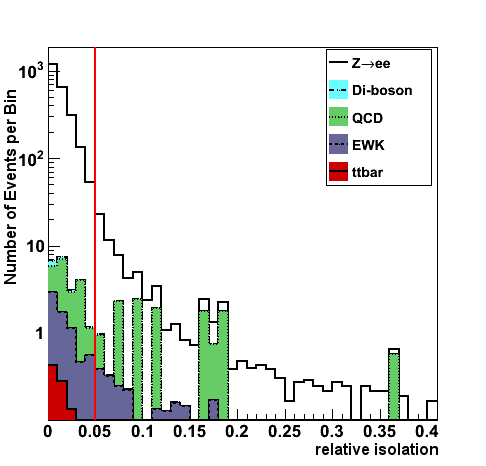
\includegraphics[width=180pt]{Figures/ecalIso-endcap-14Apr11-revised-04Jul11.png}}
  \end{center}
%  \caption[\fixspacing Electron ECAL isolation variables before respective cuts]{
%  \fixspacing Electron ECAL isolation variables before respective cuts.
  \caption[\fixspacing Electron ECAL isolation variables after \Et, conversion rejection, and tracker isolation cuts]{
  \fixspacing Electron ECAL isolation variables after \Et, 
  conversion rejection, and tracker isolation cuts.
  Relative ECAL isolation is equal to the sum of the \Et of ECAL deposits 
  in a cone around the electron, divided by the electron's \pt.
  The solid line against the white background shows the signal sample;
  the shaded areas with varied linestyles show the backgrounds.
  The vertical line shows where the cut was made.
  } 
  \label{fig:ecalElecIsoVars}
 \end{figure}



 \begin{figure}[htb]
  \begin{center}
    \subfloat[Barrel]{\label{fig:hcalBarrelElecIsoVars}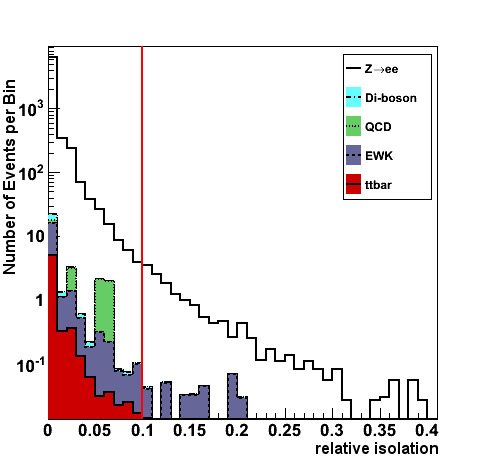
\includegraphics[width=180pt]{Figures/hcalIso-barrel-14Apr11-revised-04Jul11.png}}
    \subfloat[Endcap]{\label{fig:hcalEndcapElecIsoVars}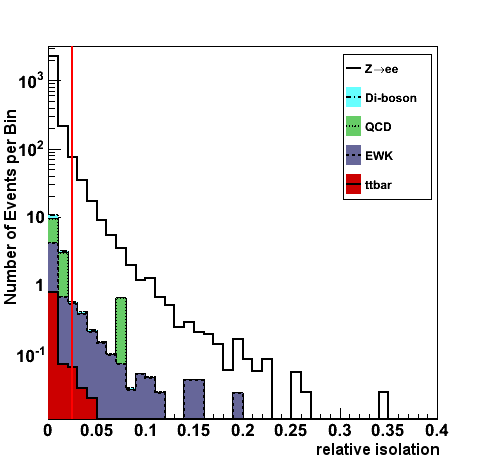
\includegraphics[width=180pt]{Figures/hcalIso-endcap-14Apr11-revised-04Jul11.png}}
  \end{center}
%  \caption[\fixspacing Electron HCAL isolation variables before respective cuts]{
%  \fixspacing Electron HCAL isolation variables before respective cuts.
  \caption[\fixspacing Electron HCAL isolation variables after \Et, conversion rejection, and tracker and ECAL isolation cuts]{
  \fixspacing Electron HCAL isolation variables after \Et, 
  conversion rejection, and tracker and ECAL isolation cuts.
  Relative HCAL isolation is equal to the sum of the \Et of HCAL deposits 
  in a cone around the electron, divided by the electron's \pt.
  The solid line against the white background shows the signal sample;
  the shaded areas with varied linestyles show the backgrounds.
  The vertical line shows where the cut was made.
  }
  \label{fig:hcalElecIsoVars}
 \end{figure}



%Figures: Reconstructed electron/photon Pt, eta, phi spectra after isolation, Fig. \ref{fig:RecoSpectraAfterEidEiso}

% \begin{figure}[htb]
%  \begin{center}
%    
\includegraphics[width=80pt, angle=90]{CMS-BW.pdf}
%  \end{center}
%  \caption[\fixspacing Reconstructed electron/photon Pt, eta, phi spectra after isolation]{\fixspacing Reconstructed electron/photon Pt, eta, phi spectra after isolation.}
%  \label{fig:RecoSpectraAfterEidEiso}
% \end{figure}


\subsubsection{Electron Identification}
\label{evSel:eid}
Several ``electron identification'' variables are used to differentiate genuine electrons  % FIXME FIND REFERENCES
from other particles or conditions that may mimic electron behavior.  
Since an electron is reconstructed from a supercluster matched to a track, it is desired that the match is a good one.
The quality of matching can be estimated by looking at measures of the distance between the two components.
The position in $ \eta $ and $ \phi $ of the supercluster is compared with 
the $ \eta $ and $ \phi $ position of the track extrapolated back to the vertex, 
with the differences being labeled \detain and \dphiin, respectively.  
It is expected that a supercluster and track from the same electron will be close together, 
so upper limits on these quantities are defined as in Table \ref{TableEidCuts}.  
Distributions of electron \detain and \dphiin, 
each plotted after 
all the 
previous selection 
%conversion and electron isolation 
steps, % (conversion rejection),
are shown in Figure~\ref{fig:dEtaInElecIdVars} and 
Figure~\ref{fig:dPhiInElecIdVars}.  

The electron's energy deposit is also expected to be narrow relative to that of a jet.
A measure of the width in the $ \eta $ direction is therefore calculated 
using the energies and positions of the individual ECAL crystals, \sieie,
and this quantity is required to be below the thresholds listed in Table \ref{TableEidCuts}.  
(The $ \phi $ direction is not examined because bremsstrahlung from the bending electron 
can cause a significant spread of the energy in $ \phi $.)  
The definition of \sieie is given in terms of the energies and $\eta$ positions of the  %% REF TALK BY SAM HARPER???
individual crystals $i$ (inclusing the seed crystal), 
as well as the energy and average position of the 
$5 \times 5$ cluster of crystals: 
\[
\sigma_{i \eta i \eta} = \sqrt{ \frac{ \sum_i{(\eta_i \times 0.0175 + \eta_{seed} - \eta_{5 \times 5}^{avg})}}{\sum_i{w_i}} }
\]
where each crystal's weight $w_i$ is given by 
\[
w_i = 4.2 + \ln{ \frac{E_i}{E_{5 \times 5}} }
\]
The \sieie distribution for electrons after all previous cuts is shown in 
Figure~\ref{fig:sieieElecIdVars}.  
In addition, an electron is expected to deposit most of its energy in the 
electromagnetic portion of the calorimeter.  
A large hadronic energy deposit is more likely to come from a jet, 
so a limit on the ratio of the energy deposit in the electromagnetic calorimeter 
to that in the hadronic calorimeter, $ H/E $, is applied (values given in the table).  
The distribution of $H/E$ for electron candidates is plotted after 
all previous selection steps in Figure~\ref{fig:hOeElecIdVars}.  


%%%% EID CUTS

\begin{table}[htbp]
%  \centering
  \begin{center}
    \caption[WP80 thresholds for electron identification variables]
    {\fixspacing WP80 thresholds for electron identification variables. 
    Each variable for a given electron 
    is required to be below the stated threshold 
    according to the electron's location in the detector. 
    Definitions of the variables are given in the text.  
    }
    \label{TableEidCuts}
    \begin{tabular}[]{ | l | c | c | }
      \hline
      Cut variable & Barrel & Endcap  \\ \hline \hline
      \sieie & 0.01 & 0.03  \\ \hline
      \dphiin & 0.06 & 0.03  \\ \hline
      \detain & 0.004 & 0.007 \\ \hline
      $ H/E $ & 0.04 & 0.025  \\
      \hline
    \end{tabular}
  \end{center}
\end{table}
%


%%%% EID DISTROS

\begin{figure}[htb]
  \centering
  %%  \begin{center}
  \subfloat[Barrel]{\label{fig:dEtaInBarrelElecIdVars}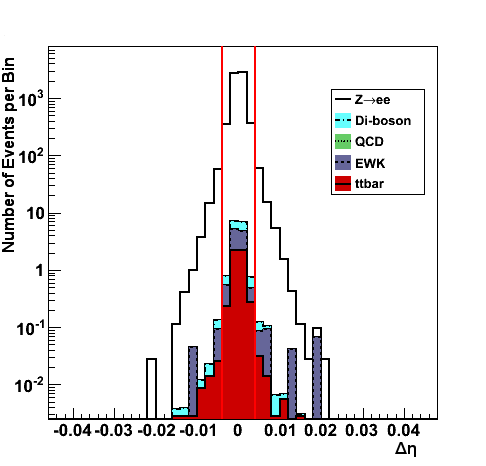
\includegraphics[width=180pt]{Figures/detain-barrel-14Apr11-revised-04Jul11.png}}
  \subfloat[Endcap]{\label{fig:dEtaInEndcapElecIdVars}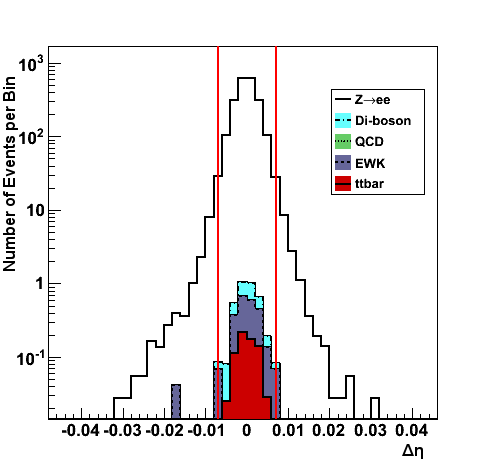
\includegraphics[width=180pt]{Figures/detain-endcap-14Apr11-revised-04Jul11.png}}
  \caption[\fixspacing \detain electron identification variables after \Et, conversion rejection, and isolation cuts]{
    \fixspacing \detain electron identification variables after \Et, conversion rejection, and isolation cuts. 
    A low \detain indicates a good match between an electron candidate's 
    supercluster and track.  
    Values shown for \subref{fig:dEtaInBarrelElecIdVars} barrel and 
    \subref{fig:dEtaInEndcapElecIdVars} endcap.
  }
  \label{fig:dEtaInElecIdVars}
\end{figure}
  
  

 \begin{figure}[htb]
  \begin{center}
    \subfloat[Barrel]{\label{fig:dPhiInBarrelElecIdVars}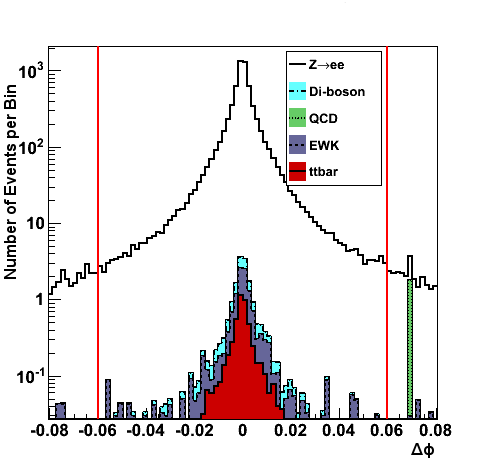
\includegraphics[width=180pt]{Figures/dphiin-barrel-14Apr11-revised-04Jul11.png}}
    \subfloat[Endcap]{\label{fig:dPhiInEndcapElecIdVars}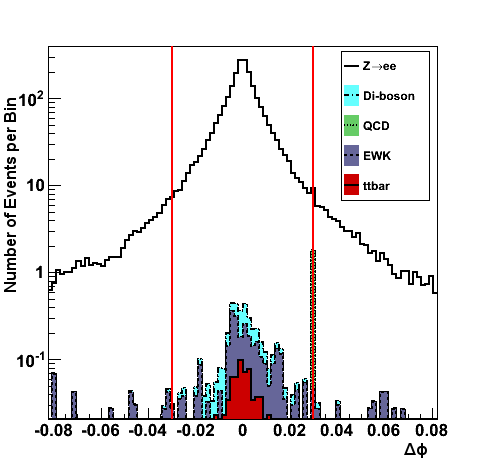
\includegraphics[width=180pt]{Figures/dphiin-endcap-14Apr11-revised-04Jul11.png}}
  \end{center}
    \caption[\fixspacing \dphiin electron identification variables after \Et, 
    conversion rejection, isolation, and \detain cuts]{
      \fixspacing \dphiin electron identification variables after \Et,
      conversion rejection, isolation, and \detain cuts.  
      A low \dphiin indicates a good match between the electron candidate's 
      supercluster and track.  
      Values shown for \subref{fig:dPhiInBarrelElecIdVars} barrel and 
      \subref{fig:dPhiInEndcapElecIdVars} endcap.
    }
  \label{fig:dPhiInElecIdVars}
 \end{figure}



 \begin{figure}[htb]
  \begin{center}
    \subfloat[Barrel]{\label{fig:sieieBarrelElecIdVars}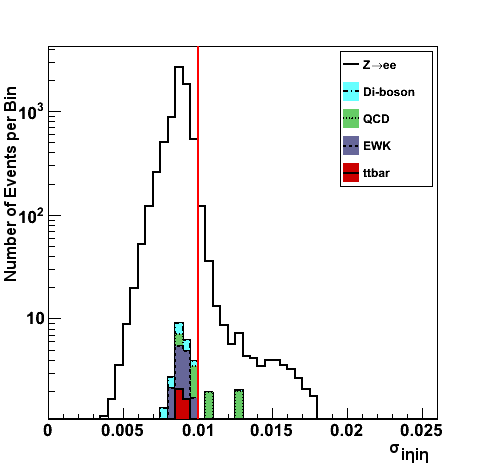
\includegraphics[width=180pt]{Figures/sieie-barrel-15Apr11-revised-04Jul11.png}}
    \subfloat[Endcap]{\label{fig:sieieEndcapElecIdVars}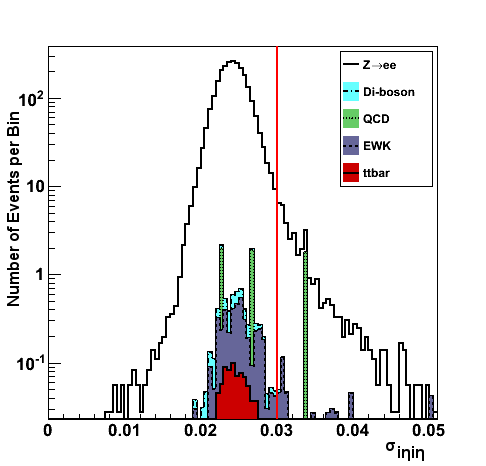
\includegraphics[width=180pt]{Figures/sieie-endcap-14Apr11-revised-04Jul11.png}}
  \end{center}
    \caption[\fixspacing \sieie electron identification variables after \Et,
    conversion rejection, isolation, \detain, and \dphiin cuts]{
      \fixspacing \sieie electron identification variables after \Et,
      conversion rejection, isolation, \detain, and \dphiin cuts.  
      \sieie is a measure of the spread of the electron candidate's energy deposite in $\eta$.  
      A true electron is expected to be relatively narrow in $\eta$.  
      Values shown for \subref{fig:sieieBarrelElecIdVars} barrel and 
      \subref{fig:sieieEndcapElecIdVars} endcap.
    }
  \label{fig:sieieElecIdVars}
 \end{figure}



 \begin{figure}[htb]
  \begin{center}
    \subfloat[Barrel]{\label{fig:hOeBarrelElecIdVars}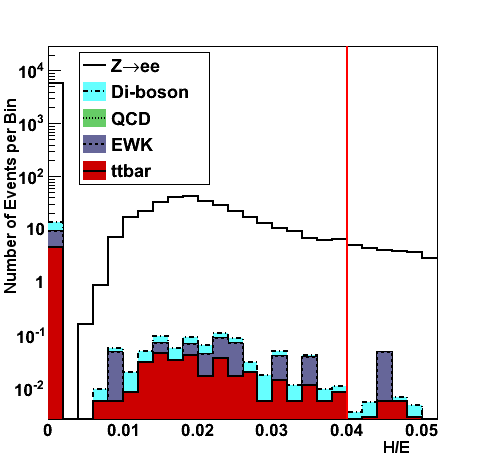
\includegraphics[width=180pt]{Figures/hoe-barrel-15Apr11-revised-04Jul11.png}}
    \subfloat[Endcap]{\label{fig:hOeEndcapElecIdVars}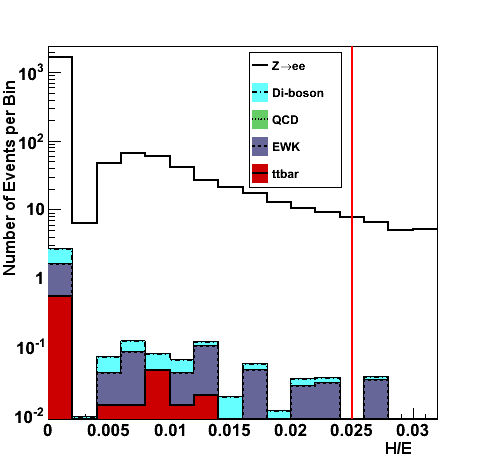
\includegraphics[width=180pt]{Figures/hoe-endcap-14Apr11-revised-04Jul11.png}}
  \end{center}
    \caption[\fixspacing H/E electron identification variables after \Et,
    conversion rejection, isolation, \detain, \dphiin, and \sieie cuts]{
      \fixspacing H/E electron identification variables after \Et,
      conversion rejection, isolation, \detain, \dphiin, and \sieie cuts.  
      H/E is the ratio of the electron candidate's energy deposited 
      in HCAL to that deposited in ECAL.  
      A true electron is expected to deposit relatively little energy in the HCAL.  
      Values shown for \subref{fig:hOeBarrelElecIdVars} barrel and 
      \subref{fig:hOeEndcapElecIdVars} endcap.
    }
  \label{fig:hOeElecIdVars}
 \end{figure}




\subsubsection{Matching Offline-Reconstructed Objects to Trigger Objects}
\label{evSel:matching}
In order to ensure that the offline-reconstructed objects being examined were also reconstructed by the trigger, 
each offline object is compared with the list of trigger objects firing a given path.  %%% L1 also, or something?!
If the offline object lies close enough to a trigger object (measured by \DR), 
it is considered to have passed the trigger.  
%All electrons used in this analysis are required to be trigger-matched in this way.  
Each event in this analysis was required to have at least one electron trigger-matched in this way, 
within a \DR distance of 0.2.  
This demonstrates that the constituent objects in the event did in fact fire an appropriate trigger.  
%According to distribution of \DR between offline and trigger objects shown in Fig. \ref{fig:TriggerObjectSelectionDeltaR}, 
%the threshold was chosen to be NUMBER.

%Figures: \DR for L1 and HLT trigger object matching, Fig. \ref{fig:TriggerObjectSelectionDeltaR}

% \begin{figure}[htb]
%  \begin{center}
%    
\includegraphics[width=360pt]{CMS-BW.pdf}
%  \end{center}
%  \caption[\fixspacing \DR for L1 and HLT trigger object matching to offline for electron selection]{\fixspacing \DR for L1 and HLT trigger object matching to offline-reconstructed objects.}
%  \label{fig:TriggerObjectSelectionDeltaR}
% \end{figure}


%\subsubsection{Electron Selection Performance} %wesley comment
%Figures: Reco PT resolution plots using MC reference for Z MC, Fig. \ref{fig:RecoPtResolution}

% \begin{figure}[htb]
%  \begin{center}
%    
\includegraphics[width=80pt, angle=90]{CMS-BW.pdf}
%  \end{center}
%  \caption[\fixspacing Reco PT resolution plots using MC reference for Z MC]{\fixspacing Reco PT resolution plots using MC reference for Z MC.}
%  \label{fig:RecoPtResolution}
% \end{figure}


\subsection{\Zee Event Selection}
\label{evSel:zee}
%trigger (including list of good triggers), mass window... that might be all

In order to be included in the final selected sample of \Zee events, 
an event must have two electrons passing the selection cuts 
described in Section~\ref{evSel:elec}.  
Only one of the electrons is required to match to a trigger object, however; 
even if only one electron fires the trigger, 
the event is kept and the trigger's purpose is served, 
and there is no 
%extra % Sridhara 
necessity for both electrons to fire the trigger.  
The two electrons are also required to have an invariant mass 
between 60 and 120 GeV; 
this defines a window around the Z mass peak at about 91 GeV.  
% TALK ABOUT INV MASS SOMEWHERE, PREV CH?

\subsubsection{Acceptance for \Zee Events}  % FIXME REFERENCE OTHER SECTION
\label{evSel:acc}
%full criteria, results
%discussion on acceptance: def, det acc vs ECAL acc, 
%systs due to theoretical vs other BUT PROB DON'T NEED SYSTS YET (do in separate ch)

% maybe end up putting def of acceptance in some more general place, like intro with that formula

The acceptance %(abbreviated $A$) 
($A$) % Sridhara
(see Section~\ref{over:xsec}) 
is the factor representing the fraction of events 
theoretically able to be detected with the given experiment.  
It includes considerations related to a particle's kinematic quantities 
(its position and momentum)
as well as to the precise definition of the signal interaction.  
In particular, the particle-detecting elements of any given 
detector, including CMS, do not fully cover the area around 
the interaction point -- 
by necessity, some of that area is taken up by the beam pipe.  
This means that any end-product particle that goes into a 
``dead'' space instead of a detecting element will not be 
detected.  
Therefore the acceptance factor takes into account the 
actual solid-angle area covered by the relevant parts of the detector.  
In addition, it is generally more difficult to distinguish 
very low-energy objects from background noise, 
so the acceptance also includes a lower limit on the 
energy of the particle.  
%It also must take into account the specific definition of the interaction.  
% 2 electrons w/in fiducial region, etc

In this analysis, the signal was defined to be those \Zee events 
whose invariant mass was between 60 and 120 GeV; 
this captures the Z peak around 91 GeV.  
The acceptance was defined as the fraction of those signal events 
whose electrons 
%end products % Sridhara
fall into the $\eta$ region used for the 
analysis, 
%|eta| < 1.4442 || 1.5660 < |eta| < 2.4, %%%%%%%%%% FORMULIFY
$|\eta| < 1.4442$ or $1.566 < |\eta| < 2.5$,
and whose transverse energies were both above 25 GeV.  
These values can also be found in Table~\ref{TableAccCuts}.  

%Make table with those criteria 

\begin{table}[htbp]
%  \centering
  \begin{center}
    \caption[Criteria for determining acceptance of \Zee events]
    {\fixspacing Criteria for determining acceptance of \Zee events.
    Acceptance is defined as the fraction of signal events 
    (within the mass window) 
    whose two electrons pass the requirements in the table.}
    \label{TableAccCuts}
    \begin{tabular}[]{ | l | c | }
      \hline
      Kinematic quantity & Requirement  \\ \hline \hline
      $\eta$ & $|\eta| < 1.4442$ or $1.566 < |\eta| < 2.5$  \\ \hline
      \Et & $ < 25 GeV$  \\ 
      \hline
    \end{tabular}
  \end{center}
\end{table}


%determined by MC estimates; room for theoretical uncertainties

Acceptance cannot be calculated from data, 
because it is impossible to know how many events were missed -- 
the only events we have are those which were not missed.  
Instead acceptance is determined by applying the defining 
criteria to a sample of simulated data, 
a sample large enough that statistical uncertainties become 
small enough to ignore.  
Since the simulated sample is expected to model real data well enough, 
this number is taken as the true acceptance for real data.  
However, 
%the information used to generate the simulated sample 
%is only a theoretical model; 
%there are many ways in which it 
the model used in simulation may actually differ slightly from 
physical reality.  
%what is used in the generation.  
These possible differences are taken into account in the 
uncertainty calculated for the acceptance, 
% OR JUST DO IT HERE??????
which will be detailed in 
Section~\ref{anMeth:SystsTheory}.  

It is also useful to combine the 
supercluster reconstruction efficiency with the acceptance. 
The supercluster reconstruction efficiency is impossible 
to determine from data for the same reason as for 
the acceptance -- 
it would require knowing about 
events that were missed, in this case 
electrons that had impacted the detector 
(specifically ECAL) but which had 
not resulted in the formation of a supercluster.  
% what about test-beam data??  I guess doesn't 
% take into account brem or pileup or non-isolation 
% or any of that stuff that could affect it
Therefore this was also determined from simulated data.  % Wesley: test beam data, but I didn't use that
Effectively it is combined with the acceptance 
by applying an additional requirement on the acceptance: 
the simulated event should have two electrons 
passing the $\eta$ and transverse energy requirements, 
and those electrons should also both be matched 
to reconstructed superclusters.  
The fraction of total events passing these combined criteria 
is referred to as 
``ECAL acceptance'' or $A_{ECAL}$.  

The pure kinematic acceptance for this analysis
was determined 
with the POW\-HEG\hyp{}generated Monte Carlo sample 
to be 
\AVal{} %0.423 %BLAH1
and the ECAL acceptance was likewise calculated as 
\AEcalVal. %0.387. %BLAH2.  
These values can also be found in Table~\ref{TableAccValues}.  


%also make table with calculated values

\begin{table}[htbp]
%  \centering
  \begin{center}
    \caption[Acceptance values for \Zee events]
    {\fixspacing Acceptance values for \Zee events. 
    Acceptance is defined as the fraction of signal events 
    whose electrons can reasonably be expected to be seen by the detector. 
    The criteria are give in Table~\ref{TableAccCuts}.}
    \label{TableAccValues}
    \begin{tabular}[]{ | l | c | c | }
      \hline
      Quantity & Value  \\ \hline \hline
      $ A $ & \AVal  \\ \hline
      $ A_{ECAL} $ & \AEcalVal  \\
      \hline
    \end{tabular}
  \end{center}
\end{table}



% MAYBE ALSO PUT THIS SECTION SOMEWHERE ELSE, even the results part

% PREV CH: DEFINE SIGNAL, BACKGROUND.  MAYBE HAVE A GLOSSARY???

\subsubsection{Efficiency of Selection for \Zee Events}
\label{evSel:eff}
%Def of efficiency (you have to know about events that were missed, could put before acc if necessary but might not be necessary...); 
%talk about different steps; 
%trigger effs done here or in trigger section (maybe easier here, because introduce T\&P here)

It is important to know how well the selection steps perform their task of 
keeping signal events;  
any signal events that are 
missed %cut out 
must be accounted for in the final 
calculation to get an accurate result.  
This factor is quantified in the efficiency, which is defined as 
the fraction of total objects or events passing a given selection. % is called 
%the selection efficiency.% and is used to 
Simulated data can be used to calculate efficiency, 
since it contains the ``truth'' information -- 
the true total number of events, 
whether or not they survive a given selection step.
However, the simulation may not correctly model some 
aspect of the real data, which would cause a discrepancy 
with the real-data efficiency 
and a corresponding inaccuracy in the final result.  
Therefore it is desirable to use so-called ``data-driven''  
methods (see also Section~\ref{over:tools}), % of determining efficiency, 
determining the efficiency as closely as possible 
using only the data itself.  
Because the truth information does not exist in real data, 
%another way must be used to determine how many 
the number of events passing or failing a given selection 
must be determined with another method.  

%Tag and Probe:  
The tag-and-probe method is used to determine the efficiency of a given set of electron selection steps.  
In this method, a set of data events is identified which appear to be good 
%Z->ee 
\Zee
candidate events.  
One of the electrons in each of these events must pass 
all selection cuts and essentially be identified as a golden electron; 
%some stringent
this is the tag.  
%The other electron must 
%pass some less stringent criteria
%be identified at least as a supercluster; 
The criteria applied to the other electron are looser: 
it is not required to pass the selection cuts being tested.  
This is the probe electron.  
The event's status as a Z candidate is determined by enforcing 
a mass window cut on the invariant mass of the tag-probe system 
(this is sufficient %(enough?) 
to select a high-purity sample of 
events in which both legs are real electrons).
% -- REFERENCE??).  
The naive selection efficiency is then given by the fraction 
of probe electrons that pass the requirement being tested.  

However, a more sophisticated analysis of the efficiency can 
be performed by fitting the invariant mass spectra of the
tag-probe pairs for both passing and failing probes to a 
lineshape representing both the signal and the background.  
Then the distribution of passing probes can be represented as 
the signal lineshape, multiplied by the efficiency and the
total number of signal events, added to the background lineshape, 
multiplied by the number of passing background events.  
The failing probe distribution can be represented in the 
analogous way, using (1 - efficiency) instead.  
From this pair of fits the total number of events as well as 
the efficiency can be extracted simultaneously.  

Several lineshapes were combined in this fit.  
The base signal lineshape was taken directly from a generator-level 
histogram of the \Zee invariant mass spectrum, %.  
which represents the true form of the invariant mass shape.  
This distribution was used together with a Gaussian distribution 
multiplied by a Crystal Ball function.  
The Gaussian has the general form 
\[
f(x) = \frac{1}{\sqrt{2\pi\sigma^2}} e^{-\frac{(x-\mu)^2}{2\sigma^2}}
\]
and takes into account the ``smearing'' effects 
of the detector resolution: 
the measured values of a quantity form a distribution 
around the ``true'' value.  
The Crystal Ball (named after the Crystal Ball collaboration) has the form
\[
f(x) = N \times 
\begin{cases}
e^{-\frac{(x-\mu)^2}{2\sigma^2}} & \text{for } \frac{x-\mu}{\sigma} > -\alpha \\
A \times \left(B - \frac{x-\mu}{\sigma} \right)^{-n} & \text{for } \frac{x-\mu}{\sigma} \leq -\alpha
\end{cases}
\]
where
\[
A = \left( \frac{n}{|\alpha|} \right)^n e^{\left( -\frac{|\alpha|^2}{2} \right)}
\]
\[
B = \frac{n}{|\alpha|} - |\alpha|
\]
The Crystal Ball function is used to 
model processes where energy may be lost 
in the measurement.  
Together they factor in the changes to the invariant mass 
spectrum due to detector limitations.  
The two shapes were combined by a process called convolution; 
the convolution of two distributions $f(x)$ and $g(x)$ is calculated by 
\[
(f * g)(x) = \int_{-\infty}^{\infty} f(y) g(x - y) dy
\]
Convolving the distributions of two independent random variables 
gives the proper combined distribution, 
as opposed to addition or multiplication.  
The background was represented by an exponential lineshape, of the form 
\[
f(x) = 
\begin{cases}
\lambda e^{-\lambda x} & \text{for } x \geq 0 \\
0 & \text{for } x < 0
\end{cases}
\]
%This was simply added to the combined signal lineshape
The parameters and relative weights of the different lineshapes 
were varied to get the combination that best fit 
the actual data distribution.  
An example of the result of this fit is shown in 
Figure~\ref{fig:TPExample}, 
for the isolation selection step in the barrel. 
Figure~\ref{fig:TPExamplePass} shows passing probes only, 
Figure~\ref{fig:TPExampleFail} shows failing probes only, 
and Figure~\ref{fig:TPExampleAll} shows the fit for all probes.  
Black points are data, the solid line is the signal lineshape, 
and the dotted line is the background lineshape.  
In the ``passing probes'' and ``all probes'' plot, 
the contribution from background is very small.  

 \begin{figure}[htb]
  \begin{center}
    \subfloat[Passing Probes]{\label{fig:TPExamplePass}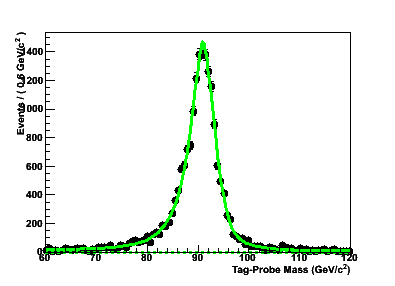
\includegraphics[width=180pt]{Figures/GsfToIso-barrel-pass-nolabel-13Jul11.png}}
    \subfloat[Failing Probes]{\label{fig:TPExampleFail}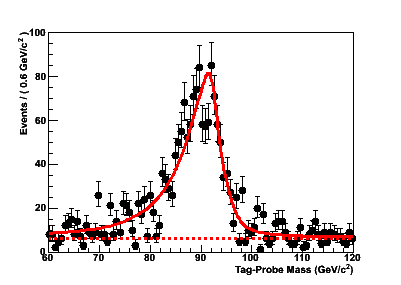
\includegraphics[width=180pt]{Figures/GsfToIso-barrel-fail-nolabel-13Jul11.png}}
    \subfloat[All Probes]{\label{fig:TPExampleAll}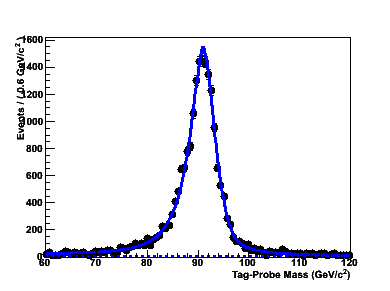
\includegraphics[width=180pt]{Figures/GsfToIso-barrel-all-nolabel-13Jul11.png}}
  \end{center}
  \caption[\fixspacing Example of tag-and-probe fits]
  {\fixspacing Example of tag-and-probe fits, 
  for the isolation selection step in the barrel: 
  \subref{fig:TPExamplePass} shows passing probes only,
  \subref{fig:TPExampleFail} shows failing probes only,
  and \subref{fig:TPExampleAll} shows the fit for all probes.
  Black points are data, the solid line is the signal lineshape,
  and the dotted line is the background lineshape.
  }
  \label{fig:TPExample}
 \end{figure}


However, the tag-and-probe may possibly introduce a bias 
into the calculation, 
in particular if observing one leg makes it more likely that 
the other leg is observed. 
For example, if the electrons are essentially back-to-back, 
one is more likely to fall within the detector coverage 
if the other one does as well.  
In addition, there is a slight discrepancy between the efficiencies 
calculated using data and those using the standard Monte Carlo sample.  
Therefore, the strategy in this analysis is to calculate the 
``true'' efficiency from the simulation sample, 
as well as the tag-and-probe efficiencies from the real data 
and simulation samples.  
The ``true'' efficiency is then corrected by the ratio of the 
data and simulation tag-and-probe efficiencies:
\[
\epsilon^{corrected} = \epsilon_{MC}^{true} \times \left( \frac{\epsilon_{data}^{T\&P}}{\epsilon_{MC}^{T\&P}} \right)
\]
This implies a certain amount of trust in the generator-level simulation of the interaction.  
The corresponding uncertainty in the efficiency due to the generator-level simulation 
is dealt with in 
Section~\ref{anMeth:SystsOtherMCEff}.  

The event selection efficiency in this analysis is determined 
by first obtaining the efficiencies of the individual 
selection steps given above. %, using the tag-and-probe method.  
This also includes the initial step of reconstructing 
the electron objects from superclusters.  
Since each selection step is applied one after the other, 
the overall selection efficiency is given by the product 
of the individual efficiencies.  
In addition, since most steps are required to apply to both electrons, 
the single-electron efficiencies of these steps 
(the result of the tag-and-probe method)
are squared to get 
the efficiency of both electrons passing that step.  
The trigger step, however, is a special case since only one electron is 
required to pass.  
In this case, the quantity used is the probability that at least 
one electron passes, 
which is equivalent to the probability both electrons fail 
subtracted from 1.  

% cute little genetics probability diagram illustration??  I kind of like that idea

The formula used to calculate the overall event selection efficiency 
from the individual step efficiencies is therefore 
\[
%BIG FAT FORMULA
%\epsilon_{total} = \epsilon_{reco}^2 \times \epsilon_{isol}^2 \times \epsilon_{ID}^2 \times \left( 1 - \left( 1 - \epsilon_{trig} \right)^2 \right)
\epsilon = \epsilon_{reco}^2 \times \epsilon_{isol}^2 \times \epsilon_{ID}^2 \times \left( 1 - \left( 1 - \epsilon_{trig} \right)^2 \right)
\]

%explain MC truth vs MC T\&P vs data T\&P (plot illustrating problem??  not really, I guess)

The efficiencies are given for each selection step in Table~\ref{TableEfficiencies} %.   %FIXME ALSO DO FOR BARREL/ENDCAP
and for all the triggers used in data individually in Table~\ref{TableTriggerEfficiencies}.  
The full event selection efficiency was calculated to be 
61.0 $\pm$ 0.5\%.  

\begin{table}[htbp]
  \begin{center}
    \caption[\fixspacing Individual efficiencies of electron selection steps]
    {\fixspacing Individual efficiencies of electron selection steps: 
    reconstruction, isolation, identification, trigger, 
    and the overall event selection efficiency.}
    \label{TableEfficiencies}
    \begin{tabular}[]{ | l | l | l | l | l | l | }
      \hline
%      STUFF \\ \hline
      Step & True MC & MC T\&P & Data T\&P & Ratio & Efficiency \\ \hline \hline
      %SC to Gsf & 0.965 & 0.972 & 0.971 $\pm$ 0.002 & 0.999 $\pm$ 0.002 & 0.964 $\pm$ 0.002 \\ \hline
%      Reconstruction & 0.965 & 0.972 & 0.971 $\pm$ 0.002 & 0.999 $\pm$ 0.002 & 0.964 $\pm$ 0.002 \\ \hline
      Reco & 0.965 & 0.972 & 0.971 $\pm$ 0.002 & 0.999 $\pm$ 0.002 & 0.964 $\pm$ 0.002 \\ \hline
      %Gsf to Iso & 0.926 & 0.927 & 0.910 $\pm$ 0.003 & 0.976 $\pm$ 0.003 & 0.905 $\pm$ 0.003 \\ \hline
%      Isolation & 0.926 & 0.927 & 0.910 $\pm$ 0.003 & 0.976 $\pm$ 0.003 & 0.905 $\pm$ 0.003 \\ \hline
      Iso & 0.926 & 0.927 & 0.910 $\pm$ 0.003 & 0.976 $\pm$ 0.003 & 0.905 $\pm$ 0.003 \\ \hline
      %Iso to Id & 0.906 & 0.907 & 0.897 $\pm$ 0.003 & 0.989 $\pm$ 0.003 & 0.896 $\pm$ 0.003 \\ \hline
%      Identification & 0.906 & 0.907 & 0.897 $\pm$ 0.003 & 0.989 $\pm$ 0.003 & 0.896 $\pm$ 0.003 \\ \hline
      ID & 0.906 & 0.907 & 0.897 $\pm$ 0.003 & 0.989 $\pm$ 0.003 & 0.896 $\pm$ 0.003 \\ \hline
      %Id to HLT & 0.959 & 0.941 & 0.972 $\pm$ 0.001 & 1.032 $\pm$ 0.001 & 0.991 $\pm$ 0.001 \\ \hline
      Trigger & 0.959 & 0.941 & 0.972 $\pm$ 0.001 & 1.032 $\pm$ 0.001 & 0.991 $\pm$ 0.001 \\ \hline \hline
      Overall & 0.654 & 0.665 & 0.621 $\pm$ 0.005 & 0.933 $\pm$ 0.007 & 0.610 $\pm$ 0.005 \\ \hline % Full Event Selection
    \end{tabular}
  \end{center}
\end{table}


%Figures: Efficiency table and supporting plots

%   * tag and probe fit plots (most in an appendix, I'd say) %FIXME

%   * BIG GIANT EFFICIENCY TABLES for each step/barrelvsendcap/datavsMC(/differentMCsamples?NO)

%   * do trigger effs separately, I guess!  Under trigger section.  or just put table here

\begin{table}[htbp]
  \begin{center}
    \caption[\fixspacing Efficiencies of trigger paths used in data]
    {\fixspacing Efficiencies of all the triggers used in data 
    as determined with the tag-and-probe method. 
    A description of the fit is given in the text.}
    \label{TableTriggerEfficiencies}
    \begin{tabular}[]{ | l | l | l | }
      \hline
      Trigger	& Efficiency & Error (fit) \\ \hline \hline
      HLT\_Photon15\_Cleaned\_L1R & 0.976 & 0.002 \\ \hline
      HLT\_Ele15\_LW\_L1R & 0.961 & 0.005 \\ \hline
      HLT\_Ele15\_SW\_L1R & 0.981 & 0.003 \\ \hline
      HLT\_Ele15\_SW\_CaloEleId\_L1R & 0.986 & 0.003 \\ \hline
      HLT\_Ele17\_SW\_CaloEleId\_L1R & 0.992 & 0.002 \\ \hline
      HLT\_Ele17\_SW\_TightEleId\_L1R & 0.973 & 0.002 \\ \hline
      HLT\_Ele17\_SW\_TighterEleIdIsol\_L1R\_v1 & 0.973 & 0.003 \\ \hline
      HLT\_Ele17\_SW\_TighterEleIdIsol\_L1R\_v2 & 0.977 & 0.002 \\ \hline
      HLT\_Ele17\_SW\_TighterEleIdIsol\_L1R\_v3 & 0.974 & 0.003 \\ \hline
      Overall & 0.9763 & 0.0009 \\ \hline
    \end{tabular}
  \end{center}
\end{table}

\clearpage
